 \documentclass[12pt,a4paper]{article}

\usepackage{graphicx}% Include figure files
\usepackage{dcolumn}% Align table columns on decimal point
\usepackage{bm}% bold math
%\usepackage{hyperref}% add hypertext capabilities
%\usepackage[mathlines]{lineno}% Enable numbering of text and display math
%\linenumbers\relax % Commence numbering lines

%\usepackage[showframe,%Uncomment any one of the following lines to test 
%%scale=0.7, marginratio={1:1, 2:3}, ignoreall,% default settings
%%text={7in,10in},centering,
%%margin=1.5in,
%%total={6.5in,8.75in}, top=1.2in, left=0.9in, includefoot,
%%height=10in,a5paper,hmargin={3cm,0.8in},
%]{geometry}

\usepackage{multicol}%Para hacer varias columnas
\usepackage{multicol,caption}
\usepackage{multirow}
\usepackage{cancel}
\usepackage{hyperref}
\hypersetup{
    colorlinks=true,
    linkcolor=blue,
    filecolor=magenta,      
    urlcolor=cyan,
}

\setlength{\topmargin}{-1.0in}
\setlength{\oddsidemargin}{-0.3pc}
\setlength{\evensidemargin}{-0.3pc}
\setlength{\textwidth}{6.75in}
\setlength{\textheight}{9.5in}
\setlength{\parskip}{0.5pc}

\usepackage[utf8]{inputenc}
\usepackage{expl3,xparse,xcoffins,titling,kantlipsum}
\usepackage{graphicx}
\usepackage{xcolor} 
\usepackage{siunitx}
\usepackage{nopageno}
\usepackage{lettrine}
\usepackage{caption}
\renewcommand{\figurename}{Figura}
\usepackage{float}
\renewcommand\refname{Bibliograf\'ia}
\usepackage{amssymb}
\usepackage{amsmath}
\usepackage[rightcaption]{sidecap}
\usepackage[spanish]{babel}

\providecommand{\abs}[1]{\lvert#1\rvert}
\providecommand{\norm}[1]{\lVert#1\rVert}
\newcommand{\dbar}{\mathchar'26\mkern-12mu d}

% CABECERA Y PIE DE PÁGINA %%%%%
\usepackage{fancyhdr}
\pagestyle{fancy}
\fancyhf{}

\begin{document}

Macías Márquez Misael Iván

\begin{enumerate}



%%%1%%%



\item Una partícula se mueve en el plano $xy$ bajo la acción de un campo de energía potencial

\begin{equation*}
    U(x,y) = \left\{\begin{matrix}
    0 & x<0 \\
    V & x> 0
    \end{matrix} \right.
\end{equation*}

\begin{enumerate}
    \item Determine al menos dos constantes de movimiento. Argumente su respuesta.
    
    \textbf{Sol:}
    
    Dadas las condiciones de nuestro sistema, su lagrangiano es
    
    \begin{equation*}
        L_{< 0} = \frac{1}{2} m (\dot{x}^2 + \dot{y}^2) 
    \end{equation*}
    
    Para $x<0$ y
    
    \begin{equation*}
        L_{ >0} = \frac{1}{2}m (\dot{x}^2 + \dot{y}^2) -V
    \end{equation*}
    
    Para $x>0$
    
    Entonces por el ejemplo $2$ de la presentación del tema 5 y como ninguna de las lagrangianas depende explícitamente de $t$, se tiene que su hamiltoniano $H$ es una constante de movimiento.
    
    Ahora como $L$ tiene simetría de traslación $(L(x+s,y+s,\dot{(x+s)},\dot{(y+s)}))=L(x,y,\dot{x},\dot{y})$ para los 2 casos, por el teorema de Noether la cantidad de movimiento total se conserva para toda $x$.
    
    
    \item Si en $t=t_0$ la partícula se encontraba en $(-a,0)$ y en el $t = t_0 + \tau$, en $(a,a)$, encuentre la posición de la partícula como función del tiempo $t$
    
    \textbf{Sol:}
    
    Aplicando las ecs. de Lagrange a los lagrangianos, llegamos a que
    
    \begin{equation*}
        \ddot{x} = 0 \hspace{1cm} \ddot{y} = 0 \hspace{1cm} \rightarrow \hspace{1cm}\dot{x} = \alpha \hspace{1cm} \dot{y} = \alpha'
    \end{equation*}
    
    con $\alpha$ y $\alpha'$ constantes, que integrando
    
    \begin{equation*}
        x = \alpha t + c \hspace{3cm} y = \alpha' t + c'
    \end{equation*}
    
    y si aplicamos lasa condiciones de los extremos $t_0$ y $t_0 + \tau$ llegamos a que
    
    \begin{equation*}
        \alpha = \frac{2a}{\tau} \hspace{3cm} \alpha' = \frac{a}{\tau}
    \end{equation*}
    
    \begin{equation*}
        c= -a (1 + \frac{2t_0}{\tau}) \hspace{3cm} c' = -\frac{at_0}{\tau}
    \end{equation*}
    
    por lo tanto la posición de la partícula en el tiempo t es
    
    \begin{equation*}
        x = \frac{2at}{\tau} -a (1 + \frac{2t_0}{\tau})
    \end{equation*}
    
    \begin{equation*}
        y = \frac{at}{\tau} -\frac{at_0}{\tau}
    \end{equation*}
    
    
    
\end{enumerate}



%%%3%%%



\item El lagrangiano de un sistema está dado por

\begin{equation*}
    L = \frac{m}{2}(a\dot{x}^2 + b \dot{x}\dot{y} + c \dot{y}^2) - \frac{k}{2}(ax^2 + bxy + cy^2)
\end{equation*}

donde $m$, $k$ son constantes positivas y $a$, $b$, $c$ son constantes arbitrarias que están sometidas a la condición $b^2 - ac = 0$.

\begin{enumerate}
    \item ¿Cuales son las ecuaciones de movimiento?
    
    \textbf{Sol:}
    
    Sustituyendo en la lagrangiana en las ecs. de Lagrange
    
    \begin{equation*}
        \frac{d}{dt}\left(\frac{\partial L}{\partial \dot{x}}\right) - \frac{\partial L}{\partial x} = 0
    \end{equation*}
    
    \begin{equation*}
        \frac{d}{dt}\left(\frac{1}{2}m (2a\dot{x}+b\dot{y})\right) + \frac{k}{2} (2ax + by)  = 0
    \end{equation*}
    
    \begin{equation*}
        (2a\ddot{x}+b\ddot{y}) + \frac{k}{m} (2ax + by)  = 0
    \end{equation*}
    
    \begin{equation*}
        \frac{d}{dt}\left(\frac{\partial L}{\partial \dot{y}}\right) - \frac{\partial L}{\partial y} = 0
    \end{equation*}
    
    \begin{equation*}
        \frac{d}{dt}\left(\frac{1}{2}m (2c\dot{y}+b\dot{x})\right) + \frac{k}{2} (2cy + bx)  = 0
    \end{equation*}
    
    \begin{equation*}
        (2c\ddot{y}+b\ddot{x}) + \frac{k}{m} (2cy + bx)  = 0
    \end{equation*}
    
    \item Encuentre una transformación de coordenadas, $x = x(\Tilde{x}, \tilde{y})$, $y = y(\Tilde{x}, \tilde{y})$, tal que las ecuaciones de movimiento resulten desacopladas en las nuevas coordenadas $\tilde{x}$ y $\tilde{y}$. ¿Cual es el significado físico de la condición $b^2 -ac = 0 $?
    
    \textbf{Sol:}
    
    Sea $\tilde{x} = 2ax + by $ y $\tilde{y}= 2cy + bx$, entonces las ecs. de movimiento son
    
    \begin{equation*}
        \ddot{\tilde{x}} + \frac{k}{m} \tilde{x} = 0
    \end{equation*}
    
    \begin{equation*}
        \ddot{\tilde{y}} + \frac{k}{m} \tilde{y} = 0
    \end{equation*}
    
    la transformación de punto se puede ver como
    
    \begin{equation*}
        \left(\begin{matrix}
        \tilde{x} \\
        \tilde{y}
        \end{matrix}\right) =
        \left(\begin{matrix}
        2a & b \\
        b & 2c
        \end{matrix}\right)
        \left(\begin{matrix}
        x \\
        y
        \end{matrix}\right)
    \end{equation*}
    
    que tiene solución si $b^2 - 4ac \neq 0 $
    

    
    
    
    \item ¿Qué sistema físico puede ser descrito por este lagrangiano?
    
    \textbf{Sol:}
    
     2 osciladores armónicos distintos
    
    
    
    
\end{enumerate}



%%%5%%%



\item Una particula se mueve bajo la acción de la gravedad sobre la cicloide

\begin{equation*}
    x = a( u + \sin{u})
\end{equation*}

\begin{equation*}
    y = a (1 - \cos{u})
\end{equation*}

con $-\pi < u < \pi$, $x$ es la coordenada horizontal y $y$ la vertical

\begin{enumerate}
    \item Halle el lagrangiano $L$
    
    \textbf{Sol:}
    
    Sabemos que la lagrangiana se describe como $L = K - U$ con $K$ la energía cinética y $U$ energía potencial, como nuestro sistema se compone de una particula bajo la acción de la gravedad, tenemos que 
    
    \begin{equation*}
        L = \frac{1}{2}m (\dot{x}^2 + \dot{y}^2) - mgy
    \end{equation*}
    
    que sustituyendo
    
    \begin{equation*}
        L = \frac{1}{2}m (a^2(1+\cos{u})^2\dot{u}^2 + a^2 \sin^2{u} \dot{u}^2) - mga (1-\cos{u})
    \end{equation*}
    
    \begin{equation*}
        = \frac{1}{2}a^2m \dot{u}^2 (\cancel{(\cos{u}^2 + \sin^2{u})} +2\cos{u} +1  ) - mga (1-\cos{u})
    \end{equation*}
    
    \begin{equation*}
        = ma^2(\cancel{\frac{2}{2}}  \dot{u}^2 (\cos{u} +1) - \frac{g}{a} (1- \cos{u}))
    \end{equation*}
    
    \begin{equation*}
        L (u,\dot{u}) = ma^2 (\cos{u} (\dot{u}^2 + \frac{g}{a}) + \dot{u}^2-\frac{g}{a})
    \end{equation*}
    
    \item Escriba la ecuación de Lagrange
    
    \textbf{Sol:}
    
    Ahora para la ec. de Lagrange para $L(u,\dot{u})$ es
    
    \begin{equation*}
        \frac{d}{dt} \left(\frac{\partial L}{\partial \dot{u}}\right) - \frac{\partial L}{\partial u} = 0
    \end{equation*}
    
    y sustituyendo el lagrangiano obtenido en a)
    
    \begin{equation*}
        \frac{\partial L}{\partial \dot{u}} = 2ma^2\dot{u} (\cos{u} + 1)  \hspace{1cm} \rightarrow \hspace{1cm} \frac{d}{dt}\left(\frac{\partial L}{\partial \dot{u}}\right) = 2ma^2\ddot{u} (\cos{u} + 1) - 2ma^2 \dot{u}^2 \sin{u} 
    \end{equation*}
    
    \begin{equation*}
        \frac{\partial L}{\partial u} = - m a^2 \sin{u} (\dot{u}^2 + \frac{g}{a})
    \end{equation*}
    
    \begin{equation*}
        \therefore \hspace{1cm} \frac{d}{dt} \left(\frac{\partial L}{\partial \dot{u}}\right) - \frac{\partial L}{\partial u}  = 2ma^2\ddot{u} (\cos{u} + 1) - 2ma^2 \dot{u}^2 \sin{u}  + m a^2 \sin{u} (\dot{u}^2 + \frac{g}{a})
    \end{equation*}
    
    \begin{equation*}
        =ma^2( 2\ddot{u} (\cos{u} + 1) -  \dot{u}^2 \sin{u}  + \frac{g}{a} \sin{u} ) = 0
    \end{equation*}
    
    o bien
    
    \begin{equation*}
        2\ddot{u} (\cos{u} + 1) -  \dot{u}^2 \sin{u}  + \frac{g}{a} \sin{u}  = 0
    \end{equation*}
    
    \item Calcule el hamiltoniano $H$ y argumente por qué $H$ es una constante de movimiento
    
    \textbf{Sol:}
    
    La expresión del hamiltoniano para $L(u,\dot{u})$ es 
    
    \begin{equation*}
        H = \frac{\partial L}{\partial \dot{u}} \dot{u} - L
    \end{equation*}
    
    \begin{equation*}
        = \cancel{2}ma^2\dot{u}^2 (\cos{u} + 1) - ma^2 (\cos{u} (\cancel{\dot{u}^2 }+ \frac{g}{a}) + \cancel{\dot{u}^2}-\frac{g}{a})
    \end{equation*}
    
    \begin{equation*}
        H(u,\dot{u}) = ma^2(\dot{u}^2 (\cos{u}+1) - \frac{g}{a}(\cos{u} -1))
    \end{equation*}
    
    ahora como vimos en el ejemplo 2 de la presentación de teorema de conservación, si $L$ no depende explícitamente de $t$ entonces su hamiltoniano es una cantidad conservada por lo que el hamiltoniano anterior debe ser una cantidad conservada.
    
\end{enumerate}





%%%6%%%



\item Dos partículas de masa $m$ y $M$ están unidas por un hilo que pasa por un agujero practicado en una mesa, tal que $M$ está restringida a moverse (sin fricción) sobre la superficie horizontal de la mes, mientras $m$ cuelga del hilo y sólo se mueve a lo largo de una recta vertical, como se ilustra en la figura. La gravedad actúa en dirección vertical.

\begin{figure}[h!]
    \centering
    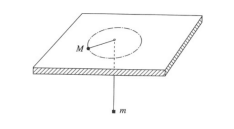
\includegraphics{2.PNG}
\end{figure}

\begin{enumerate}
    \item ¿Cuantos grados de libertad tiene el sistema?¿Cual serian un conjunto de coordenadas generalizadas?
    
    \textbf{Sol:}
    
    Primero coloquemos nuestro origen sobre el agujero, como tenemos 2 partículas y 4 restricciones holonómicas ($z_M = 0$, $x_m = y_m = 0$ y $v_M = -v_m$) entonces los grados de libertad son  $f= 3(2)-4 = 2$.
    
    Un conjunto de coordenadas generalizadas útiles para este problema son las polares ($\theta$, $r$)
    
    \item Escriba el lagrangiano y las ecuaciones de Lagrange del sistema
    
    \textbf{Sol:}
    
    Sea $a$ la longitud del hilo, $r$ la longitud de la masa $M$ al agujero y $z$ la distancia de la masa $m$ al agujero ($a = r+z$), entonces en coordenadas polares/cilíndricas en cartesianas se tiene que
    
    \begin{equation*}
        x_M = r \cos{\theta}\hspace{3cm} y_M = r \sin{\theta}
    \end{equation*}
    
    \begin{equation*}
        z_m =- z = (r-a) 
    \end{equation*}
    
    entonces el lagrangiano es
    
    \begin{equation*}
        L = \frac{1}{2} m (\cancel{\dot{x}_{m}^{2}} + \cancel{\dot{y}_{m}^{2}}+ \dot{z}_m^2) + \frac{1}{2} M (\dot{x}_M^2 + \dot{y}_M^2 + \cancel{\dot{z}_M^2}) - mg(a-r)
    \end{equation*}
    
    \begin{equation*}
        =\frac{1}{2} m \dot{r}^2 + \frac{1}{2} M ((\dot{r} \cos{\theta}-r\sin{\theta}\dot{\theta})^2 + (\dot{r}\sin{\theta}+r\cos{\theta}\dot{\theta})^2) - mg(a-r)
    \end{equation*}
    
    \begin{equation*}
        =\frac{1}{2} m \dot{r}^2 + \frac{1}{2} M ((\dot{r}^2 + r^2 \dot{\theta}^2) - mg(a-r)
    \end{equation*}
    
    \begin{equation*}
        L(r,\dot{r},\dot{\theta}) = \frac{1}{2}(m+M) \dot{r}^2 + \frac{1}{2}M r^2 \dot{\theta}^2 - mg (a-r)
    \end{equation*}
    
    que sustituyendo en las ecs. de Lagrange
    
    \begin{equation*}
        \frac{d}{dt}\left(\frac{\partial L}{\partial \dot{r}}\right) - \frac{\partial L}{\partial r} = 0
    \end{equation*}
    
    \begin{equation*}
        \frac{d}{dt}\left((m+M)\dot{r}\right) - Mr\dot{\theta}^2+mg = 0
    \end{equation*}
    
    \begin{equation*}
        (m+M)\ddot{r} - Mr\dot{\theta}^2+mg = 0
    \end{equation*}
    
    \begin{equation*}
        \frac{d}{dt}\left(\frac{\partial L}{\partial \dot{\theta}}\right) -\cancel{ \frac{\partial L}{\partial \theta}}= 0
    \end{equation*}
    
    \begin{equation*}
        \frac{d}{dt}\left(Mr^2\dot{\theta}\right)= 0
    \end{equation*}
    
    
    \item ¿Existe alguna coordenada cíclica? En caso que su respuesta sea afirmativa, diga la cantidad correspondiente que se conserva y significado físico
    
    \textbf{Sol:}
    
    Como $L$ no depende de $\theta$, entonces $\frac{\partial L}{\partial \theta} = 0$ por lo que $\theta$ es una variable cíclica, esto también nos dice que $Mr^2\dot{\theta}$ es una cantidad conservada (como se puede ver en la ec. de Lagrange para $\theta$)
    
    Ya que el momento de $M$ es perpendicular a $\mathbf{r}$ por ser un movimiento circular,
    
    \begin{equation*}
        M r^2 \dot{\theta} = r(Mr \omega) = |\mathbf{r}||\mathbf{p}| \sin{\pi/2} = \mathbf{r} \times \mathbf{p}
    \end{equation*}
    
    Que es el momento angular de $M$ así que la cantidad conservada es el momento angular de la partícula con masa $M$, que esta cantidad se conserve significa que el torque para la partícula de masa $M$ es nulo.
    
    \item Reducir el problema a una sola ecuación diferencial de segundo orden y obtener una primera integral de la ecuación.
    
    \textbf{Sol:}
    
    Juntando las ecs. de Lagrange 
    
    \begin{equation*}
        (m+M)\ddot{r} - Mr\dot{\theta}^2+mg =  \frac{d}{dt}\left(Mr^2\dot{\theta}\right)
    \end{equation*}
    
    
    
    \item Discutir si es posible que la partícula $M$ se mantenga realizando un movimiento circular
    
    \textbf{Sol:}
    
    
    
    
    Para mantener un movimiento circular para la partícula $M$ se debe tener que la fuerza sobre $m$ debido a la gravedad debe ser igual a la fuerza ficticia centrífuga sobre $M$ a causa de la rotación por lo que
    
    \begin{equation*}
        M \omega^2 r = mg
    \end{equation*}
    
    \begin{equation*}
        \omega = \sqrt{\frac{mg}{Mr}}
    \end{equation*}
    
\end{enumerate}
    
    
\end{enumerate}

\end{document}